\documentclass{beamer}

\usefonttheme{professionalfonts} % using non standard fonts for beamer
\usefonttheme{serif} % default family is serif

%\usepackage{hyperref}

%\usepackage{minted}

\usepackage{animate}

\usepackage{graphicx}

\def\Put(#1,#2)#3{\leavevmode\makebox(0,0){\put(#1,#2){#3}}}

\usepackage{color}

\usepackage{tikz}

\usepackage{amssymb}

\usepackage{enumerate}


\newcommand\blfootnote[1]{%

  \begingroup

  \renewcommand\thefootnote{}\footnote{#1}%

  \addtocounter{footnote}{-1}%

  \endgroup

}

\makeatletter

%%%%%%%%%%%%%%%%%%%%%%%%%%%%%% Textclass specific LaTeX commands.

 % this default might be overridden by plain title style

 \newcommand\makebeamertitle{\frame{\maketitle}}%

 % (ERT) argument for the TOC

 \AtBeginDocument{%

   \let\origtableofcontents=\tableofcontents

   \def\tableofcontents{\@ifnextchar[{\origtableofcontents}{\gobbletableofcontents}}

   \def\gobbletableofcontents#1{\origtableofcontents}

 }

%%%%%%%%%%%%%%%%%%%%%%%%%%%%%% User specified LaTeX commands.

\usetheme{Malmoe}

% or ...

\useoutertheme{infolines}

\addtobeamertemplate{headline}{}{\vskip2pt}



\setbeamercovered{transparent}

% or whatever (possibly just delete it)

\makeatother

\begin{document}
\title[SDCEL report]{Geoinformatica paper extension}
\author[AC]{}
\institute[UCR]{University of California, Riverside}
\makebeamertitle
\newif\iflattersubsect

% \AtBeginSection[] {
%   \begin{frame}<beamer>
%     \frametitle{Outline} 
%     \tableofcontents[currentsection]  
%   \end{frame}
%   \lattersubsectfalse
% }

\AtBeginSubsection[] {
  \begin{frame}<beamer>
    \frametitle{Outline} 
    \tableofcontents[currentsubsection]  
  \end{frame}
}

\begin{frame}{So far...}
  \begin{itemize}
    \item I had some troubles with Bronw's k-d tree to define the cell boundaries in real data (also dealing with float-point data)...
    \item Sedona's k-d tree already integrate this quite well...
    \item Brown algorithm was useful to understand better sedona's one and I was able to move part of the optimization to a custom code...
  \end{itemize}
\end{frame}

\begin{frame}{So far...}
  \begin{itemize}
    \item I think that given a representative sample it is possible to detect unbalanced cells and compute an initial set of intervals for optimization...
    \item Once we feed the tree to assign each point we could update the interval accordingly...
    \item It should give us some advantage because we save subsequent sorting and we will have a set of intervals ready for optimization...
  \end{itemize}
\end{frame}

%\begin{frame}{Some invalids polygons...}
%    \centering 
    %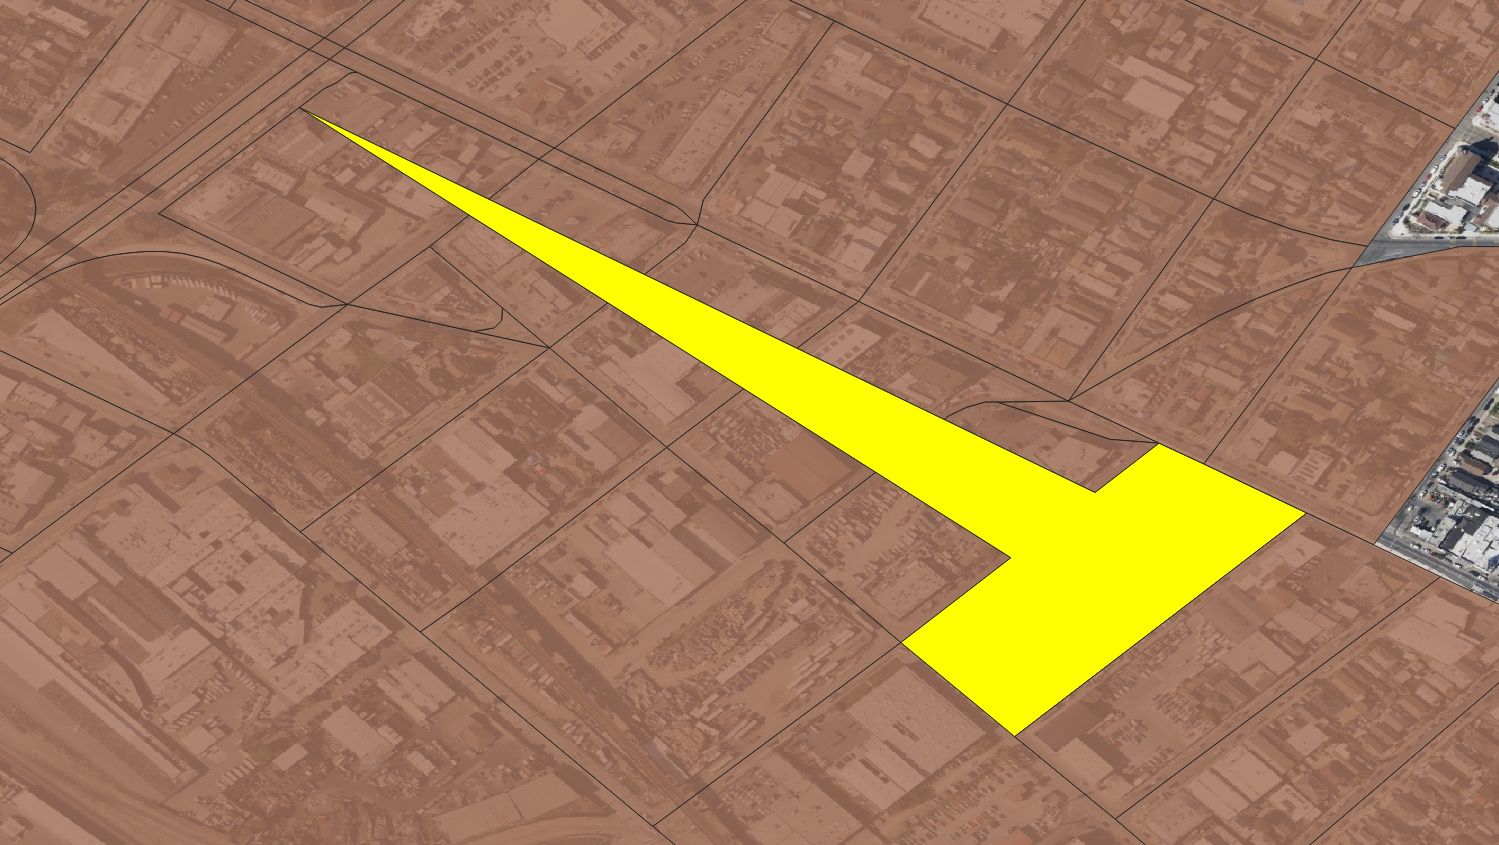
\includegraphics[width=0.8\textwidth]{figures/artifact02}
%\end{frame}

\end{document}
